\section{Verwandte Arbeiten} \label{sec:VerwandteArbeiten}
In diesem Abschnitt werden verwandte Arbeiten vorgestellt, die auch das Layoutproblem betrachten.
Außerdem will ich auch konkrete Tools anschauen, die Metriken visualisieren und deren Ansätze betrachten.


Ziel der Suche:
ich will 2d layouts finden, die geeignet sein könnten, um Software-Qualitätsmetriken zu visualisieren in 2.5D.

Wie entscheide ich, ob ein layout geeignet ist:
- Es sollte eine Art von Metrik oder Wert darstellen können.
- Es sollte eine Art von Layout haben, dass die Struktur der Hierarchie darstellt.
- Es sollte ins drei dimensionale extrahierbar sein.
- Es soll auch ohne spezielle Einfärbung im 2D funktionieren - eventuell nur die ordner einfärben

Wir wollen möglichst viele Layouts finden, auch welche, die nicht direkt für Software-Qualitätsmetriken gedacht sind oder die nicht direkt für das extrudieren ins drei dimensionale gedacht sind, aber die trotzdem geeignet sein könnten.
Deswegen suchen wir auf folgenden Seiten, die 1. nicht wissenschaftlich sind, da wir nach tools suchen und 2. allgemein sind für visualisierungen:

Wissenschaftlich:
Google Scholar und IEEE
Tools:
Google und GitHub

Hierarchical data visualization methods
Space-filling Hierarchy Visualization
Software Quality Visualization
Alternative Tree Structure Visualization
context display hierarchy visualizations


Nochmal mehr nach schlagworten schauen
Bei cascaded, was für schlagwörter - in welchem kontext wurde es veröffentlicht
Software Qualitätsvis mehr einbrigen in die Suche - eher auf diese Niesche eingehen

Methodik auch so beschreiben, wie es wirklich war ... wie wurden die ersten paper gefunden (durch "zufall") um das zu festigen und abzusichern noch eine strukturierte Methodik 

























\subsection{visualization Libraries} \ref{sec:VisualizationLibraries}
Wir schauen uns verschiedene bekannte Open-source Visualisierungsbibliotheken. Oft haben diese eine gute Übersicht über verschiedene Visualisierungen. Der Vorteil ist natürlich dass man diese dann direkt auch verwenden kann, ohne selbst zu implementieren oder man kann den code nehmen und selbst anpassen.

Man muss mit einer gewissen kreativität an die sache heran gehen, es werden alle Visualisierungen betrachtet, es kann natürlich sein ,dass jemand noch mehr finden würde, wir suchen aber hier die geeignetsten heraus

Für die Github suche nutzen wir eine Offene List von visualierungstools \cite{awesome_2025}.

wir schauen uns d3.js an, die bekannteste javascript Visualisierungsbibliothek:
es gibt extra 


Zuerst seaborn in der galery: \cite{seaborngalery}
\begin{figure}
    \centering
    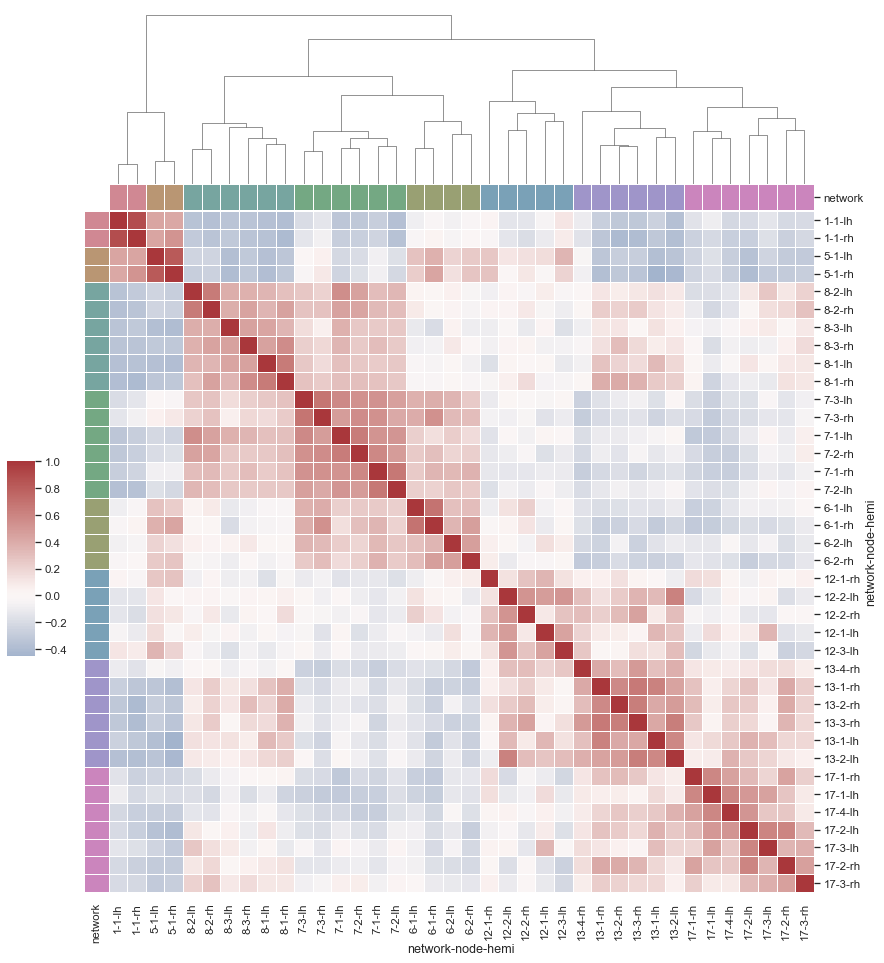
\includegraphics[width=0.8\textwidth]{images/structureHeatmapSeaborn.png}
    \caption{Beispiel für eine Heatmap aus der Seaborn Galery \cite{seaborngalery}.}
    \label{fig:seabornHeatmap} 
\end{figure}
Seaborn bietet keine Visualierungen, die gut für unseren zweck geeignet sein könnten. Das was noch am nächsten kommt, wäre eine heatmap, wie in Abbildung \ref{fig:seabornHeatmap} zu sehen, die zusätlich über ein Baumdiagram informationen über die Struktur darstellt, wie in der Einleitung aber schon gesagt, ist das nicht wirklich geeignet, da es hierbei für große Daten probleme gibt mit baumdigrammen und diese unübersichtlich werden.
außerdem sollen die diagramme auch möglichst einfach sein.


\subsection{layouts}

So etwas ähnliches auch sagen:
A number of other hierarchy visualization techniques have been
developed [18, 23, 29, 32], including space-filling visualizations
like step trees [6], Voronoi treemaps [2] and generalized treemaps
[34]. Although relevant to hierarchy visualization, we pursue
contributions that are sufficiently distinct from such work that we
do not dwell on extensive comparisons. \cite{lu2008cascaded}

\subsubsection{Treemap layouts}
Wir suchen hierfür speziell nach layouts die abstände haben. die meisten treemap layouts haben keine abstände, wodurch bei der extrusion ins drei dimensionale und ohne farbgebung die Struktur der Hierarchie nicht mehr erkennbar ist. Deswegen wird speziell nach treemap layouts gesucht, die abstände haben und die Struktur der Hierarchie darstellen.


Es gibt bisher noch zu wenige ARbeiten, die sich mit dieser Frage beschäftigen. (Oder eigentlich gibt es nur eine die wirklich in die richtung geht - mehr dann bei verwandte arbeiten)


\cite{lu2008cascaded}:
Hao Lü and James Fogarty stellten in ihrem Paper \textit{Cascaded Treemaps:
Examining the Visibility and Stability of Structure in Treemaps}\cite{lu2008cascaded} fest: \enquote{an important limitation of treemaps is
the difficulty of discerning the structure of a hierarchy}\cite[1]{lu2008cascaded} Das stellt im Grunde das Problem von Treemaps dar, welches auch algorithmisch nicht einfach gelöst werden kann (siehe Abschnitt \ref{sec:TreemapProblem}). Die Idee ist anders als bei Nested Ansätzen die Kindknoten nicht einfach in den Elternknoten zu zeichnen, sondern sie leicht versetzt \textit{über} dem Elternknoten zu zeichnen (siehe Abbildung \ref{fig:cascaded}). Dadurch soll weniger Platz verloren gehen und es entsteht ein leichter 3D-Effekt.

\begin{figure}
    \centering
    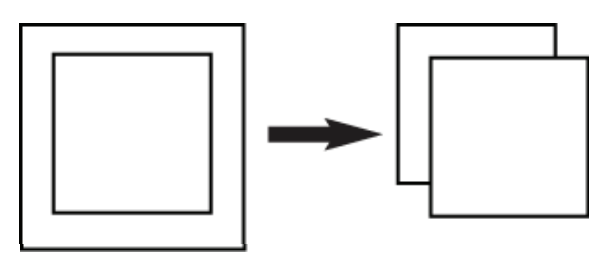
\includegraphics[width=0.8\textwidth]{images/cascaded.png}
    \caption{Links beispielhaf der Nested treemaps Ansatz, bei dem der Kindknoten einfach in dem Elternknoten gezeichnet wird. Rechts der Cascaded Treemap Ansatz, bei dem der Kindknoten als rechteck leicht versetzt nach rechts unten \textit{über} dem Elternknoten gezeichnet wird. Abbildung aus \cite[3]{lu2008cascaded}.}
    \label{fig:cascaded}
\end{figure}

Sie stellen in ihrem Paper auch fest, dass manche Knoten verschwinden können, da der Platz der für Beschriftung und abstände benötigt wird, beim Layoutschritt nicht berücksichtigt werden kann. Sie stellen einen Zwei Schrittigen ansatz vor, der im ersten schritt mit den squarify algorithmus \cite{bruls2000squarified} das layout erstellt. 
Im zweiten Schritt wird dann die Größe, aber nicht die Platzierung der Knoten angepasst. 
indem der Abstand und platz für Beschriftung berücksichtigt wird. Das Problem von verschwindenden Knoten wird dadurch nicht komplett gelöst, aber Knoten verschwinden nur noch, wenn der Platz für die Beschriftung und den Abstand größer ist als der zur Verfügung stehende Platz. Die Autoren geben leider keinen Pseudo-Code für die exakte implementierung an, weshalb es schwer ist die genaue berechnung nachzuvollziehen und Unterschiede und Vor- und Nachteile zu den Implementierungen in diser Arbeit aufzuzeigen.
Sie beschreiben ihren Schritt wie folgt: 
\begin{quote}
    The function then computes how much vertical space is needed for offsets [...]. The remaining space is for the content of the treemap, and so the layout function gives each side of the split the space computed as necessary for [...] offsets as well as a portion of the remaining content space based on the relative weights of nodes on each side of the split. The layout procedure is then ready to recurse on both sides of the split, as it knows how much space will be used by [...] offsets and has ensured that the remaining space is appropriately divided by node weight. \cite[6]{lu2008cascaded}
\end{quote} (FÜR MICH: das ist quasi simple-increase mit scaling)
Sie berechnen also die Fläche, für jeden Knoten neu. An jeder Teilungs-Kante, die kante an der ein Knoten geteilt wurde (entweder horizontal oder vertikal) - im grunde werden sich immer die reihen angeschaut. Wird dann der Platz berechnet, der für die Abstände benötigt wird. Anschließend wird der Platz für die Knoten berechnet, indem der Platz für die Abstände von der Gesamtfläche abgezogen wird. Dadurch wird sichergestellt, dass jeder Knoten genug Platz für die Abstände hat. Dennoch kann es passieren, dass Knoten verschwinden, wenn der Platz für die Abstände größer ist als der Platz, der für die Knoten zur Verfügung steht.
Obwohl der Code nicht verfügbar ist, wird doch allein bei der Beschreibung ein Nachteil deutlich: Es wird an jeder Reihen-Kante nur der Platz mit in die Berechnung einbezogen, der senkrecht zu der Kante steht. In Abbildung \ref{fig:cascadedBadExample} für deutlich, dass der Algorithmus für den Bereich über von der Kante benauso viel Platz für die Abstände berechnet, wie für den Bereicht unter der Kante, weil eben nur der Platz senkrecht zur Kante betrachtet wird. Und das obwohl offentlich die Roten Rechtecke zusammen viel Mehr platz für die Abstände benötigen würden, als das Gelbe Rechteck alleine. 
Das Grundlegende Problem, welches wir zuvor beschrieben haben (siehe Abschnitt \ref{sec:TreemapProblem}), ist also nicht gelöst. 

\begin{figure}
    \centering
    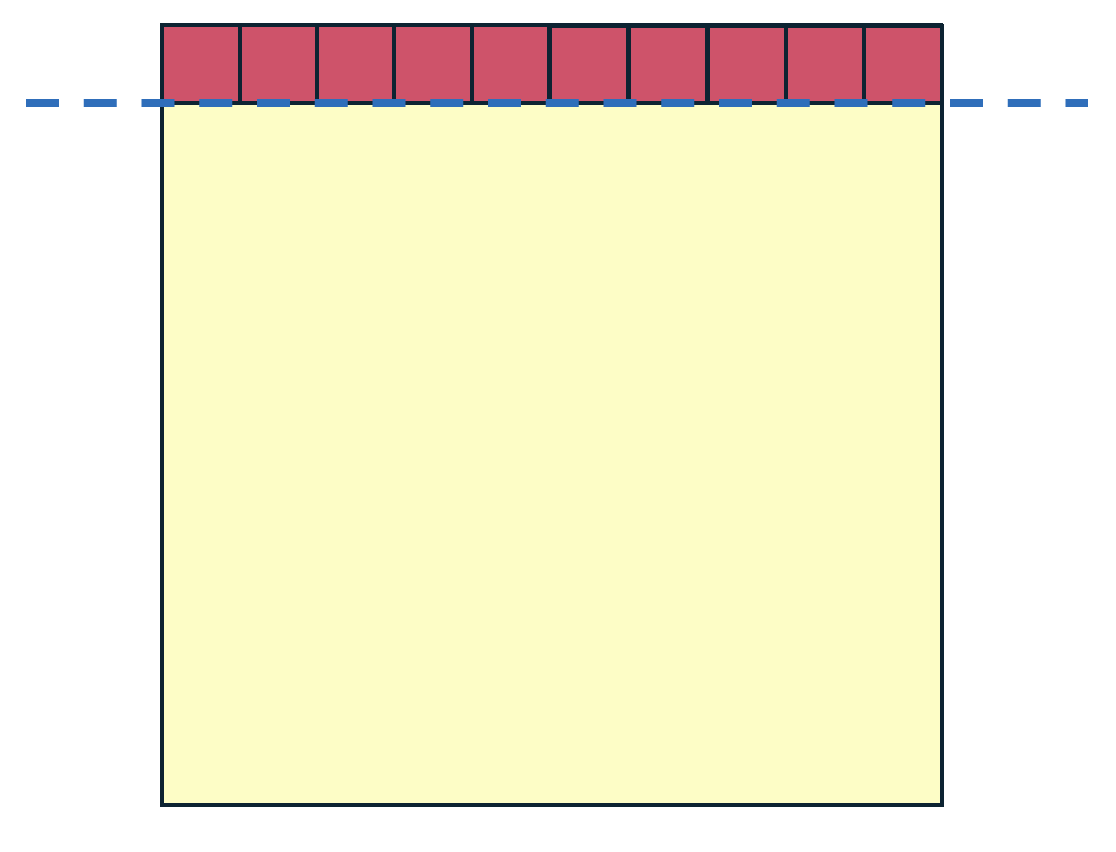
\includegraphics[width=0.8\textwidth]{images/cascadedBadExample.png}
    \caption{Beispiel für eine für den Cascaded Treemap Algorithmus schlechte Rechteck-Konstelation}
    \label{fig:cascadedBadExample}
\end{figure}

Interessant ist, dass die Autoren keine verbesserung in der Gewicht zu Größe relation feststellen konnten. (Ich vermute, dass das daran liegt, dass die Berechnung der neuen Größen für die Knoten nicht optimal ist) 
Eine verbesserung konnten sie nur bei relativ kleinen Knoten feststellen, was auch klar ist, da bei den ansätzen zuvor die Abstände (da diese ja absolut sind und bei jedem knoten gleich) die Größe von kleinen Knoten viel stärker beeinflussen, als die Größe von großen. Sie vermuten auch, dass das an Ihrem Ansatz speziell liegen könnte und fordern noch weitere research in diesem Bereich.
Sie vermuten außerdem, dass speziell bei Tiefen Hierarchien, die Abweichung von Größe zu Gewicht größer wird.  

Eine ähnliche implementierungen untersuchen wir in Abschnitt HIER EINFÜGEN und zeigen genau auf, warum dieser Ansatz große Schwächen hat. bzw 
Am ehesten ist dieser Ansatz wahrscheinlich mit dem Simple-Increase Ansatz mit Scaling und festen Knoten zu vergleichen, nur mit dem Umterschied, dass die kompletten abstände betrachtet werden und diese betrachtung nur einmalig nach dem ersten squarify Layout Schritt durchgeführt wird (was auch in dem casced paper angemerkt wurde, dass das einmalige berechnen der Abstände eine mögliche Optimierung ihres Ansatzes wäre \cite[6]{lu2008cascaded}).





Die Autoren des ursprungs squarify Algorithmus \cite{bruls2000squarified} stellen in einem anderen Paper \cite{cushionTreemaps} eine Idee vor, um Struktur ohne Änderung des Layouts darzustellen undzwar mit Schatten (siehe Abbildung \ref{fig:cushion}). Dabei bekommt jeder Knoten, egal ob Eltern- oder Kindknoten, einen Innenrenschatten, wodurch die Struktur der Knoten sichbar wird.

\begin{figure}
    \centering
    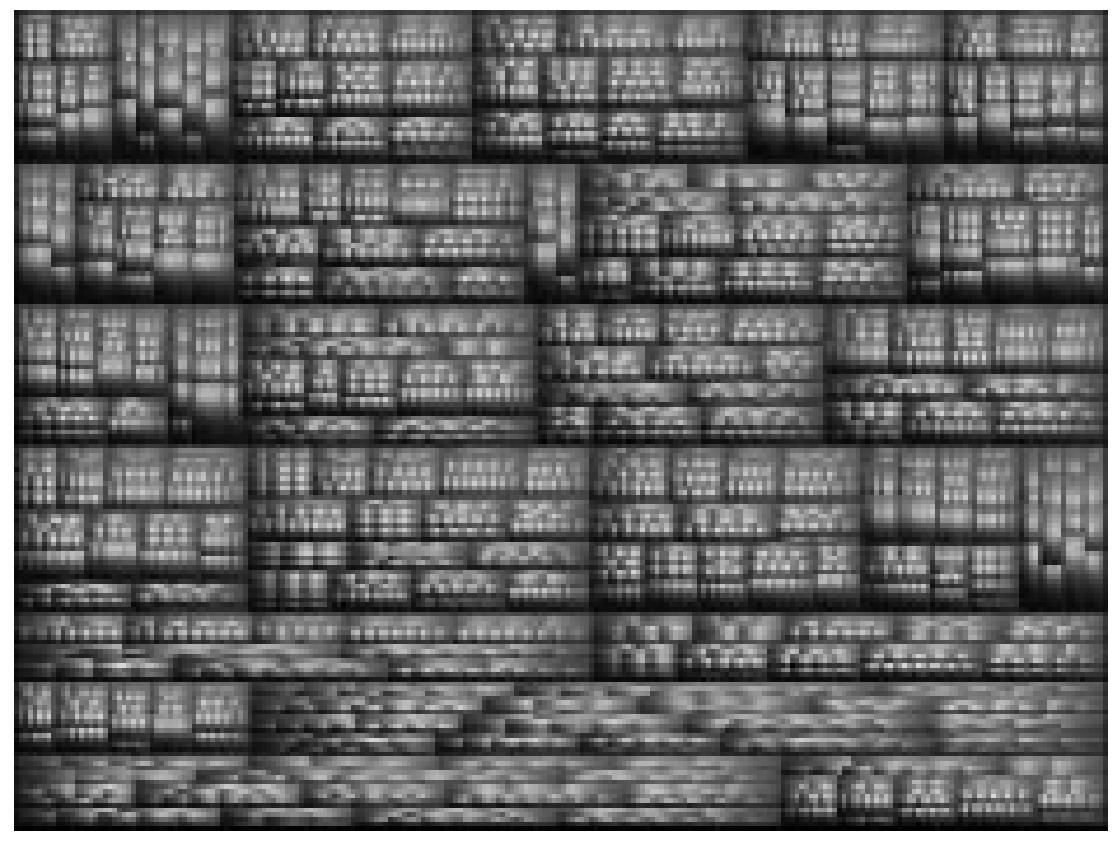
\includegraphics[width=0.8\textwidth]{images/cushionTreemap.png}
    \caption{Beispiel für eine Cushion Treemap \cite[4]{cushionTreemaps}}
    \label{fig:cushion}
\end{figure}

Peter Demian und Renate Fruchter stellen die Idee vor dass dickere outlines he höher der Knoten ist auch die Struktur verdeutlichen können. 

Nicholas Kong et al schlagen vor verschiedene Umriss dicken zu nutzen um die Struktur der Knoten darzustellen.\cite{2010-perception-treemaps} (siehe Abbildung \ref{fig:thickOutline}).

% \begin{figure}
%     \centering
%     \includegraphics[width=0.8\textwidth]{images/thickOutline.png}
%     \caption{Beispiel für eine Treemap mit verschieden dicken outlines, die die Struktur verdeutlichen sollen. Abbildung aus \cite[1]{2010-perception-treemaps}}
%     \label{fig:thickOutline}
% \end{figure}

Scheibel et al. stellen in ihrem Paper \textit{Survey of treemap layout algorithms}\cite{scheibel2020survey} eine Übersicht über die verschiedenen Treemap Layout Algorithmen vor. Sie unterscheiden zwischen den verschiedenen Ansätzen. 

Sie kategorieren die verschiedenen Ansätze in 4 Kategorien: Art der Aufteilung, zusätzliche Attribute, Layout Form und Referenzraum Dimension. 
Uns interresiert hier besonders das zusätzliche Attribut der "Werte" und die Dimension 2D (wie in Abschnitt \ref{sec:Problemstellung} beschrieben).
Arten der Aufteilung sind: Packing und splitting. Packing ist dabei die Idee, die Knoten so zu packen, dass sie möglichst wenig Platz verbrauchen und splitting ist die Idee Knoten in kleinere Knoten zu unterteilen. Alle in den Grundlagen (Abschnit \ref{sec:Treemap}) vorgestellten Algorithmen sind also splitting Algorithmen.
Sie stellen vier Layout Formen vor: Kreisförmig, rechteckig, konvex und nicht konvex. Alle in den Grundlagen vorgestellten Algorithmen sind rechteckige Layouts.
Von den untersuchten 81 Algorithmen sind 54 rechteckige Layouts und 58 splitting Algorithmen. Der in dieser ARbeit speziell untersuchte Treemap Algorithmus passt also genau in die Kategorie der meist verwendeten Ansätze.

\smallskip

\subsection{Was suchen wir} 
Wir suchen paper oder tools, die metriken oder andere werte/attribute darstellen.
Diese Darstellungen sollten entweder space filling sein oder zumindest eine Art von Layout haben, dass die Struktur der Hierarchie darstellt.
Die Darstellungen sollten ins drei dimensionale extrahierbar sein. 
Die Darstellungen werden dann etweder in die kategorie "squarified treemap" oder "andere" eingeordnet.



\subsection{Tools}
